\documentclass[]{article}
\usepackage{lmodern}
\usepackage{amssymb,amsmath}
\usepackage{ifxetex,ifluatex}
\usepackage{fixltx2e} % provides \textsubscript
\ifnum 0\ifxetex 1\fi\ifluatex 1\fi=0 % if pdftex
  \usepackage[T1]{fontenc}
  \usepackage[utf8]{inputenc}
\else % if luatex or xelatex
  \ifxetex
    \usepackage{mathspec}
  \else
    \usepackage{fontspec}
  \fi
  \defaultfontfeatures{Ligatures=TeX,Scale=MatchLowercase}
\fi
% use upquote if available, for straight quotes in verbatim environments
\IfFileExists{upquote.sty}{\usepackage{upquote}}{}
% use microtype if available
\IfFileExists{microtype.sty}{%
\usepackage{microtype}
\UseMicrotypeSet[protrusion]{basicmath} % disable protrusion for tt fonts
}{}
\usepackage[margin=1in]{geometry}
\usepackage{hyperref}
\hypersetup{unicode=true,
            pdftitle={C8\_W4\_Project},
            pdfauthor={Tom},
            pdfborder={0 0 0},
            breaklinks=true}
\urlstyle{same}  % don't use monospace font for urls
\usepackage{color}
\usepackage{fancyvrb}
\newcommand{\VerbBar}{|}
\newcommand{\VERB}{\Verb[commandchars=\\\{\}]}
\DefineVerbatimEnvironment{Highlighting}{Verbatim}{commandchars=\\\{\}}
% Add ',fontsize=\small' for more characters per line
\usepackage{framed}
\definecolor{shadecolor}{RGB}{248,248,248}
\newenvironment{Shaded}{\begin{snugshade}}{\end{snugshade}}
\newcommand{\KeywordTok}[1]{\textcolor[rgb]{0.13,0.29,0.53}{\textbf{#1}}}
\newcommand{\DataTypeTok}[1]{\textcolor[rgb]{0.13,0.29,0.53}{#1}}
\newcommand{\DecValTok}[1]{\textcolor[rgb]{0.00,0.00,0.81}{#1}}
\newcommand{\BaseNTok}[1]{\textcolor[rgb]{0.00,0.00,0.81}{#1}}
\newcommand{\FloatTok}[1]{\textcolor[rgb]{0.00,0.00,0.81}{#1}}
\newcommand{\ConstantTok}[1]{\textcolor[rgb]{0.00,0.00,0.00}{#1}}
\newcommand{\CharTok}[1]{\textcolor[rgb]{0.31,0.60,0.02}{#1}}
\newcommand{\SpecialCharTok}[1]{\textcolor[rgb]{0.00,0.00,0.00}{#1}}
\newcommand{\StringTok}[1]{\textcolor[rgb]{0.31,0.60,0.02}{#1}}
\newcommand{\VerbatimStringTok}[1]{\textcolor[rgb]{0.31,0.60,0.02}{#1}}
\newcommand{\SpecialStringTok}[1]{\textcolor[rgb]{0.31,0.60,0.02}{#1}}
\newcommand{\ImportTok}[1]{#1}
\newcommand{\CommentTok}[1]{\textcolor[rgb]{0.56,0.35,0.01}{\textit{#1}}}
\newcommand{\DocumentationTok}[1]{\textcolor[rgb]{0.56,0.35,0.01}{\textbf{\textit{#1}}}}
\newcommand{\AnnotationTok}[1]{\textcolor[rgb]{0.56,0.35,0.01}{\textbf{\textit{#1}}}}
\newcommand{\CommentVarTok}[1]{\textcolor[rgb]{0.56,0.35,0.01}{\textbf{\textit{#1}}}}
\newcommand{\OtherTok}[1]{\textcolor[rgb]{0.56,0.35,0.01}{#1}}
\newcommand{\FunctionTok}[1]{\textcolor[rgb]{0.00,0.00,0.00}{#1}}
\newcommand{\VariableTok}[1]{\textcolor[rgb]{0.00,0.00,0.00}{#1}}
\newcommand{\ControlFlowTok}[1]{\textcolor[rgb]{0.13,0.29,0.53}{\textbf{#1}}}
\newcommand{\OperatorTok}[1]{\textcolor[rgb]{0.81,0.36,0.00}{\textbf{#1}}}
\newcommand{\BuiltInTok}[1]{#1}
\newcommand{\ExtensionTok}[1]{#1}
\newcommand{\PreprocessorTok}[1]{\textcolor[rgb]{0.56,0.35,0.01}{\textit{#1}}}
\newcommand{\AttributeTok}[1]{\textcolor[rgb]{0.77,0.63,0.00}{#1}}
\newcommand{\RegionMarkerTok}[1]{#1}
\newcommand{\InformationTok}[1]{\textcolor[rgb]{0.56,0.35,0.01}{\textbf{\textit{#1}}}}
\newcommand{\WarningTok}[1]{\textcolor[rgb]{0.56,0.35,0.01}{\textbf{\textit{#1}}}}
\newcommand{\AlertTok}[1]{\textcolor[rgb]{0.94,0.16,0.16}{#1}}
\newcommand{\ErrorTok}[1]{\textcolor[rgb]{0.64,0.00,0.00}{\textbf{#1}}}
\newcommand{\NormalTok}[1]{#1}
\usepackage{graphicx,grffile}
\makeatletter
\def\maxwidth{\ifdim\Gin@nat@width>\linewidth\linewidth\else\Gin@nat@width\fi}
\def\maxheight{\ifdim\Gin@nat@height>\textheight\textheight\else\Gin@nat@height\fi}
\makeatother
% Scale images if necessary, so that they will not overflow the page
% margins by default, and it is still possible to overwrite the defaults
% using explicit options in \includegraphics[width, height, ...]{}
\setkeys{Gin}{width=\maxwidth,height=\maxheight,keepaspectratio}
\IfFileExists{parskip.sty}{%
\usepackage{parskip}
}{% else
\setlength{\parindent}{0pt}
\setlength{\parskip}{6pt plus 2pt minus 1pt}
}
\setlength{\emergencystretch}{3em}  % prevent overfull lines
\providecommand{\tightlist}{%
  \setlength{\itemsep}{0pt}\setlength{\parskip}{0pt}}
\setcounter{secnumdepth}{0}
% Redefines (sub)paragraphs to behave more like sections
\ifx\paragraph\undefined\else
\let\oldparagraph\paragraph
\renewcommand{\paragraph}[1]{\oldparagraph{#1}\mbox{}}
\fi
\ifx\subparagraph\undefined\else
\let\oldsubparagraph\subparagraph
\renewcommand{\subparagraph}[1]{\oldsubparagraph{#1}\mbox{}}
\fi

%%% Use protect on footnotes to avoid problems with footnotes in titles
\let\rmarkdownfootnote\footnote%
\def\footnote{\protect\rmarkdownfootnote}

%%% Change title format to be more compact
\usepackage{titling}

% Create subtitle command for use in maketitle
\providecommand{\subtitle}[1]{
  \posttitle{
    \begin{center}\large#1\end{center}
    }
}

\setlength{\droptitle}{-2em}

  \title{C8\_W4\_Project}
    \pretitle{\vspace{\droptitle}\centering\huge}
  \posttitle{\par}
    \author{Tom}
    \preauthor{\centering\large\emph}
  \postauthor{\par}
      \predate{\centering\large\emph}
  \postdate{\par}
    \date{April 16, 2020}


\begin{document}
\maketitle

\section{Practical Machine Learning
Project}\label{practical-machine-learning-project}

The goal of this project is to predict the manner in which they did the
exercise. This is the ``classe'' variable in the training set. Will also
use our prediction model to predict 20 different test cases.

\begin{center}\rule{0.5\linewidth}{\linethickness}\end{center}

\subsection{Background}\label{background}

Using devices such as Jawbone Up, Nike FuelBand, and Fitbit it is now
possible to collect a large amount of data about personal activity
relatively inexpensively. These type of devices are part of the
quantified self movement - a group of enthusiasts who take measurements
about themselves regularly to improve their health, to find patterns in
their behavior, or because they are tech geeks. One thing that people
regularly do is quantify how much of a particular activity they do, but
they rarely quantify how well they do it. In this project, your goal
will be to use data from accelerometers on the belt, forearm, arm, and
dumbell of 6 participants. They were asked to perform barbell lifts
correctly and incorrectly in 5 different ways. More information is
available from the website here:
\url{http://groupware.les.inf.puc-rio.br/har} (see the section on the
Weight Lifting Exercise Dataset).

Read more: \url{http://groupware.les.inf.puc-rio.br/har\#ixzz3xsbS5bVX}

\begin{center}\rule{0.5\linewidth}{\linethickness}\end{center}

\subsection{Preparing Data}\label{preparing-data}

Below we begin by loading in the data

\begin{Shaded}
\begin{Highlighting}[]
\KeywordTok{library}\NormalTok{(knitr)}
\end{Highlighting}
\end{Shaded}

\begin{verbatim}
## Warning: package 'knitr' was built under R version 3.5.3
\end{verbatim}

\begin{Shaded}
\begin{Highlighting}[]
\KeywordTok{library}\NormalTok{(caret)}
\end{Highlighting}
\end{Shaded}

\begin{verbatim}
## Warning: package 'caret' was built under R version 3.5.3
\end{verbatim}

\begin{verbatim}
## Loading required package: lattice
\end{verbatim}

\begin{verbatim}
## Warning: package 'lattice' was built under R version 3.5.3
\end{verbatim}

\begin{verbatim}
## Loading required package: ggplot2
\end{verbatim}

\begin{verbatim}
## Warning: package 'ggplot2' was built under R version 3.5.3
\end{verbatim}

\begin{Shaded}
\begin{Highlighting}[]
\KeywordTok{library}\NormalTok{(rpart)}
\KeywordTok{library}\NormalTok{(rpart.plot)}
\end{Highlighting}
\end{Shaded}

\begin{verbatim}
## Warning: package 'rpart.plot' was built under R version 3.5.3
\end{verbatim}

\begin{Shaded}
\begin{Highlighting}[]
\KeywordTok{library}\NormalTok{(rattle)}
\end{Highlighting}
\end{Shaded}

\begin{verbatim}
## Warning: package 'rattle' was built under R version 3.5.3
\end{verbatim}

\begin{verbatim}
## Rattle: A free graphical interface for data science with R.
## Version 5.3.0 Copyright (c) 2006-2018 Togaware Pty Ltd.
## Type 'rattle()' to shake, rattle, and roll your data.
\end{verbatim}

\begin{Shaded}
\begin{Highlighting}[]
\KeywordTok{library}\NormalTok{(randomForest)}
\end{Highlighting}
\end{Shaded}

\begin{verbatim}
## Warning: package 'randomForest' was built under R version 3.5.3
\end{verbatim}

\begin{verbatim}
## randomForest 4.6-14
\end{verbatim}

\begin{verbatim}
## Type rfNews() to see new features/changes/bug fixes.
\end{verbatim}

\begin{verbatim}
## 
## Attaching package: 'randomForest'
\end{verbatim}

\begin{verbatim}
## The following object is masked from 'package:rattle':
## 
##     importance
\end{verbatim}

\begin{verbatim}
## The following object is masked from 'package:ggplot2':
## 
##     margin
\end{verbatim}

\begin{Shaded}
\begin{Highlighting}[]
\KeywordTok{library}\NormalTok{(gbm)}
\end{Highlighting}
\end{Shaded}

\begin{verbatim}
## Warning: package 'gbm' was built under R version 3.5.3
\end{verbatim}

\begin{verbatim}
## Loaded gbm 2.1.5
\end{verbatim}

\begin{Shaded}
\begin{Highlighting}[]
\KeywordTok{library}\NormalTok{(AppliedPredictiveModeling)}
\end{Highlighting}
\end{Shaded}

\begin{verbatim}
## Warning: package 'AppliedPredictiveModeling' was built under R version 3.5.3
\end{verbatim}

\begin{Shaded}
\begin{Highlighting}[]
\KeywordTok{library}\NormalTok{(corrplot)}
\end{Highlighting}
\end{Shaded}

\begin{verbatim}
## Warning: package 'corrplot' was built under R version 3.5.3
\end{verbatim}

\begin{verbatim}
## corrplot 0.84 loaded
\end{verbatim}

\begin{Shaded}
\begin{Highlighting}[]
\KeywordTok{set.seed}\NormalTok{(}\DecValTok{12345}\NormalTok{)}
\end{Highlighting}
\end{Shaded}

\begin{Shaded}
\begin{Highlighting}[]
\CommentTok{# URL for the data download}
\NormalTok{train_data <-}\StringTok{ "http://d396qusza40orc.cloudfront.net/predmachlearn/pml-training.csv"}
\NormalTok{test_data  <-}\StringTok{ "http://d396qusza40orc.cloudfront.net/predmachlearn/pml-testing.csv"}

\CommentTok{# training and test data sets downloadd }
\NormalTok{training <-}\StringTok{ }\KeywordTok{read.csv}\NormalTok{(}\KeywordTok{url}\NormalTok{(train_data))}
\NormalTok{testing  <-}\StringTok{ }\KeywordTok{read.csv}\NormalTok{(}\KeywordTok{url}\NormalTok{(test_data))}

\CommentTok{# breaking up the training and test data sets by taking 70% of the data for training }
\NormalTok{inTrain  <-}\StringTok{ }\KeywordTok{createDataPartition}\NormalTok{(training}\OperatorTok{$}\NormalTok{classe, }\DataTypeTok{p=}\FloatTok{0.7}\NormalTok{, }\DataTypeTok{list=}\OtherTok{FALSE}\NormalTok{)}
\NormalTok{train_set <-}\StringTok{ }\NormalTok{training[inTrain, ]}
\NormalTok{test_set  <-}\StringTok{ }\NormalTok{training[}\OperatorTok{-}\NormalTok{inTrain, ]}
\KeywordTok{dim}\NormalTok{(train_set)}
\end{Highlighting}
\end{Shaded}

\begin{verbatim}
## [1] 13737   160
\end{verbatim}

\begin{Shaded}
\begin{Highlighting}[]
\KeywordTok{dim}\NormalTok{(test_set)}
\end{Highlighting}
\end{Shaded}

\begin{verbatim}
## [1] 5885  160
\end{verbatim}

Both created datasets have 160 variables. Those variables have plenty of
NA, that can be removed with the cleaning procedures below. The Near
Zero variance (NZV) variables are also removed and the ID variables as
well.

The training and test data are loaded above and a training set has been
created to assist in our creation of a model for the test data set. We
see that both the training and test sets hav 160 variables, but
differing number of values from the data partition. The basic set up has
been completed and next we will look to clean the data by removing NA's
and the variables with near zero variance as well.

\subsubsection{Cleaning the Data}\label{cleaning-the-data}

Removal of near zero variance variables

\begin{Shaded}
\begin{Highlighting}[]
\CommentTok{# Variables with nearly zero variance removed in both training and test sts}
\NormalTok{NZV <-}\StringTok{ }\KeywordTok{nearZeroVar}\NormalTok{(train_set)}
\NormalTok{train_set <-}\StringTok{ }\NormalTok{train_set[, }\OperatorTok{-}\NormalTok{NZV]}
\NormalTok{test_set  <-}\StringTok{ }\NormalTok{test_set[, }\OperatorTok{-}\NormalTok{NZV]}
\KeywordTok{dim}\NormalTok{(train_set)}
\end{Highlighting}
\end{Shaded}

\begin{verbatim}
## [1] 13737   106
\end{verbatim}

\begin{Shaded}
\begin{Highlighting}[]
\KeywordTok{dim}\NormalTok{(test_set)}
\end{Highlighting}
\end{Shaded}

\begin{verbatim}
## [1] 5885  106
\end{verbatim}

Removal of variables that mostly contain NA's as they would have not
have significant impact

\begin{Shaded}
\begin{Highlighting}[]
\CommentTok{# variables that mostly contain NA are removed }
\NormalTok{NA_Var    <-}\StringTok{ }\KeywordTok{sapply}\NormalTok{(train_set, }\ControlFlowTok{function}\NormalTok{(x) }\KeywordTok{mean}\NormalTok{(}\KeywordTok{is.na}\NormalTok{(x))) }\OperatorTok{>}\StringTok{ }\FloatTok{0.95}
\NormalTok{train_set <-}\StringTok{ }\NormalTok{train_set[, NA_Var}\OperatorTok{==}\OtherTok{FALSE}\NormalTok{]}
\NormalTok{test_set  <-}\StringTok{ }\NormalTok{test_set[, NA_Var}\OperatorTok{==}\OtherTok{FALSE}\NormalTok{]}
\KeywordTok{dim}\NormalTok{(train_set)}
\end{Highlighting}
\end{Shaded}

\begin{verbatim}
## [1] 13737    59
\end{verbatim}

\begin{Shaded}
\begin{Highlighting}[]
\KeywordTok{dim}\NormalTok{(test_set)}
\end{Highlighting}
\end{Shaded}

\begin{verbatim}
## [1] 5885   59
\end{verbatim}

Removal of variables that only act as identification

\begin{Shaded}
\begin{Highlighting}[]
\CommentTok{# Columns 1 to 5 removed as they are only identification variables }
\NormalTok{train_set <-}\StringTok{ }\NormalTok{train_set[, }\OperatorTok{-}\NormalTok{(}\DecValTok{1}\OperatorTok{:}\DecValTok{5}\NormalTok{)]}
\NormalTok{test_set  <-}\StringTok{ }\NormalTok{test_set[, }\OperatorTok{-}\NormalTok{(}\DecValTok{1}\OperatorTok{:}\DecValTok{5}\NormalTok{)]}
\KeywordTok{dim}\NormalTok{(train_set)}
\end{Highlighting}
\end{Shaded}

\begin{verbatim}
## [1] 13737    54
\end{verbatim}

\begin{Shaded}
\begin{Highlighting}[]
\KeywordTok{dim}\NormalTok{(test_set)}
\end{Highlighting}
\end{Shaded}

\begin{verbatim}
## [1] 5885   54
\end{verbatim}

Our two step clean up of the data sets has reduced our variable counts
down to only 54 variables, but the number of observations remains the
same. Now that our data has been cleaned we can proceed to analysis.

\begin{center}\rule{0.5\linewidth}{\linethickness}\end{center}

\subsection{Correlation}\label{correlation}

Prior to the start of the modeling process we take a look at the
correlation plot below to see which variables to see which variables
have the strongest correlations. Darker colors indicate stronger
correlations

\begin{Shaded}
\begin{Highlighting}[]
\NormalTok{cor_mat <-}\StringTok{ }\KeywordTok{cor}\NormalTok{(train_set[, }\OperatorTok{-}\DecValTok{54}\NormalTok{])}
\KeywordTok{corrplot}\NormalTok{(cor_mat, }\DataTypeTok{order =} \StringTok{"FPC"}\NormalTok{, }\DataTypeTok{method =} \StringTok{"color"}\NormalTok{, }\DataTypeTok{type =} \StringTok{"lower"}\NormalTok{, }\DataTypeTok{tl.cex =} \FloatTok{0.8}\NormalTok{, }\DataTypeTok{tl.col =} \KeywordTok{rgb}\NormalTok{(}\DecValTok{0}\NormalTok{, }\DecValTok{0}\NormalTok{, }\DecValTok{0}\NormalTok{))}
\end{Highlighting}
\end{Shaded}

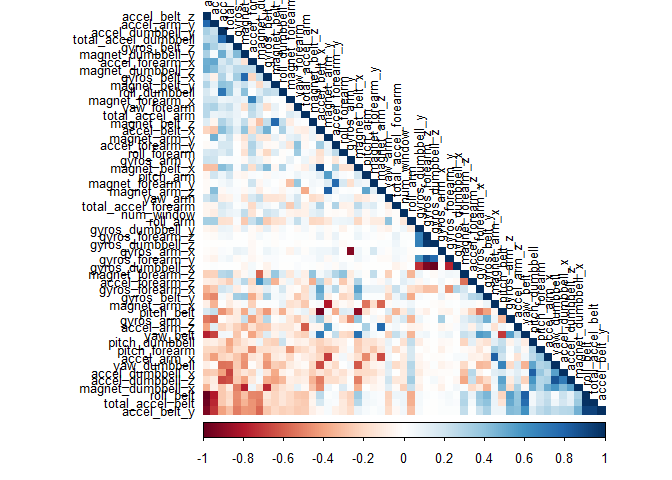
\includegraphics{C8_W4_Course_Project_files/figure-latex/Correlate-1.pdf}

In order to see the highest variable correlations we run the code below
and create a cutoff of 0.75

\begin{Shaded}
\begin{Highlighting}[]
\NormalTok{high_corr =}\StringTok{ }\KeywordTok{findCorrelation}\NormalTok{(cor_mat, }\DataTypeTok{cutoff =} \FloatTok{0.75}\NormalTok{)}
\KeywordTok{names}\NormalTok{(train_set)[high_corr]}
\end{Highlighting}
\end{Shaded}

\begin{verbatim}
##  [1] "accel_belt_z"      "roll_belt"         "accel_belt_y"     
##  [4] "total_accel_belt"  "accel_dumbbell_z"  "accel_belt_x"     
##  [7] "pitch_belt"        "magnet_dumbbell_x" "accel_dumbbell_y" 
## [10] "magnet_dumbbell_y" "accel_arm_x"       "accel_dumbbell_x" 
## [13] "accel_arm_z"       "magnet_arm_y"      "magnet_belt_z"    
## [16] "accel_forearm_y"   "gyros_forearm_y"   "gyros_dumbbell_x" 
## [19] "gyros_dumbbell_z"  "gyros_arm_x"
\end{verbatim}

\begin{center}\rule{0.5\linewidth}{\linethickness}\end{center}

\subsection{Modeling}\label{modeling}

For the predictive model building we will incorporate the use of three
different methods applied on the training data set to help us determine
the best one to apply. The preferred method will be chosen based on
which results in the highest accuracy on the test data set. The three
methods include: Random Forests, Decision Tree, and Generalized Boosted
Modeling.

\subsubsection{Method 1: Random Forest}\label{method-1-random-forest}

Below is the code for the first attempted method, Random Forest. The
method is selected, a model is fit on the training data and then applied
to the test set. A confusion matrix shows the prediction and a plot of
the matrix helps us visualize and see the accuracy.

\begin{Shaded}
\begin{Highlighting}[]
\CommentTok{# Model 1}
\KeywordTok{set.seed}\NormalTok{(}\DecValTok{12345}\NormalTok{)}
\NormalTok{control_RF <-}\StringTok{ }\KeywordTok{trainControl}\NormalTok{(}\DataTypeTok{method=}\StringTok{"cv"}\NormalTok{, }\DataTypeTok{number=}\DecValTok{3}\NormalTok{, }\DataTypeTok{verboseIter=}\OtherTok{FALSE}\NormalTok{)}
\NormalTok{modFit_RF <-}\StringTok{ }\KeywordTok{train}\NormalTok{(classe }\OperatorTok{~}\StringTok{ }\NormalTok{., }\DataTypeTok{data=}\NormalTok{train_set, }\DataTypeTok{method=}\StringTok{"rf"}\NormalTok{, }\DataTypeTok{trControl=}\NormalTok{control_RF)}
\NormalTok{modFit_RF}\OperatorTok{$}\NormalTok{finalModel}
\end{Highlighting}
\end{Shaded}

\begin{verbatim}
## 
## Call:
##  randomForest(x = x, y = y, mtry = param$mtry) 
##                Type of random forest: classification
##                      Number of trees: 500
## No. of variables tried at each split: 27
## 
##         OOB estimate of  error rate: 0.2%
## Confusion matrix:
##      A    B    C    D    E  class.error
## A 3904    1    0    0    1 0.0005120328
## B    6 2649    2    1    0 0.0033860045
## C    0    4 2391    1    0 0.0020868114
## D    0    0    7 2245    0 0.0031083481
## E    0    0    0    5 2520 0.0019801980
\end{verbatim}

\begin{Shaded}
\begin{Highlighting}[]
\CommentTok{# prediction on test dataset with confusion matrix }
\NormalTok{pred_RF <-}\StringTok{ }\KeywordTok{predict}\NormalTok{(modFit_RF, }\DataTypeTok{newdata=}\NormalTok{test_set)}
\NormalTok{Matrix_RF <-}\StringTok{ }\KeywordTok{confusionMatrix}\NormalTok{(pred_RF, test_set}\OperatorTok{$}\NormalTok{classe)}
\NormalTok{Matrix_RF}
\end{Highlighting}
\end{Shaded}

\begin{verbatim}
## Confusion Matrix and Statistics
## 
##           Reference
## Prediction    A    B    C    D    E
##          A 1674    5    0    0    0
##          B    0 1133    4    0    0
##          C    0    1 1022    7    0
##          D    0    0    0  957    4
##          E    0    0    0    0 1078
## 
## Overall Statistics
##                                           
##                Accuracy : 0.9964          
##                  95% CI : (0.9946, 0.9978)
##     No Information Rate : 0.2845          
##     P-Value [Acc > NIR] : < 2.2e-16       
##                                           
##                   Kappa : 0.9955          
##                                           
##  Mcnemar's Test P-Value : NA              
## 
## Statistics by Class:
## 
##                      Class: A Class: B Class: C Class: D Class: E
## Sensitivity            1.0000   0.9947   0.9961   0.9927   0.9963
## Specificity            0.9988   0.9992   0.9984   0.9992   1.0000
## Pos Pred Value         0.9970   0.9965   0.9922   0.9958   1.0000
## Neg Pred Value         1.0000   0.9987   0.9992   0.9986   0.9992
## Prevalence             0.2845   0.1935   0.1743   0.1638   0.1839
## Detection Rate         0.2845   0.1925   0.1737   0.1626   0.1832
## Detection Prevalence   0.2853   0.1932   0.1750   0.1633   0.1832
## Balanced Accuracy      0.9994   0.9969   0.9972   0.9960   0.9982
\end{verbatim}

\begin{Shaded}
\begin{Highlighting}[]
\CommentTok{# visualization of confusion matrix }
\KeywordTok{plot}\NormalTok{(Matrix_RF}\OperatorTok{$}\NormalTok{table, }\DataTypeTok{col =}\NormalTok{ Matrix_RF}\OperatorTok{$}\NormalTok{byClass, }
     \DataTypeTok{main =} \KeywordTok{paste}\NormalTok{(}\StringTok{"Random Forest - Accuracy ="}\NormalTok{, }\KeywordTok{round}\NormalTok{(Matrix_RF}\OperatorTok{$}\NormalTok{overall[}\StringTok{'Accuracy'}\NormalTok{], }\DecValTok{4}\NormalTok{)))}
\end{Highlighting}
\end{Shaded}

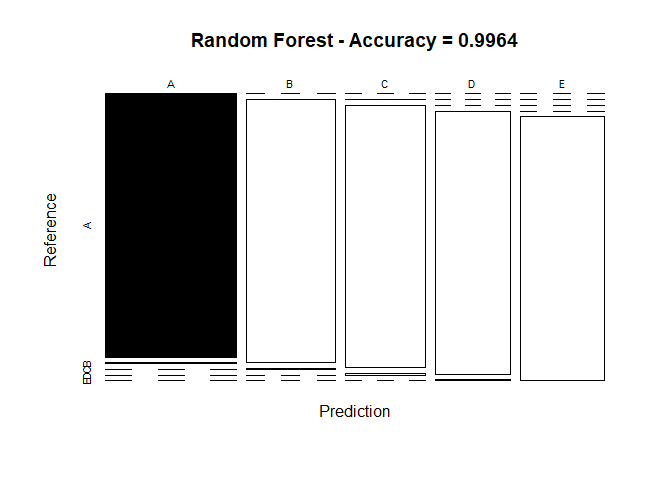
\includegraphics{C8_W4_Course_Project_files/figure-latex/RF_plot-1.pdf}

As a result of our Random Forest method we see that the resulting
Accuracy is at 0.9983. This is a strong level of accuracy, but we
continue on with the next two methods to see if they are even better.

\begin{center}\rule{0.5\linewidth}{\linethickness}\end{center}

\subsubsection{Method 2: Decision Tree}\label{method-2-decision-tree}

The second method used is the decision tree.

\begin{Shaded}
\begin{Highlighting}[]
\KeywordTok{set.seed}\NormalTok{(}\DecValTok{12345}\NormalTok{)}
\NormalTok{modFit_DT <-}\StringTok{ }\KeywordTok{rpart}\NormalTok{(classe }\OperatorTok{~}\StringTok{ }\NormalTok{., }\DataTypeTok{data=}\NormalTok{train_set, }\DataTypeTok{method=}\StringTok{"class"}\NormalTok{)}
\KeywordTok{fancyRpartPlot}\NormalTok{(modFit_DT)}
\end{Highlighting}
\end{Shaded}

\begin{verbatim}
## Warning: labs do not fit even at cex 0.15, there may be some overplotting
\end{verbatim}

\includegraphics{C8_W4_Course_Project_files/figure-latex/model_2-1.pdf}

\begin{Shaded}
\begin{Highlighting}[]
\CommentTok{# prediction on test dataset with confusion matrix }
\NormalTok{pred_DT <-}\StringTok{ }\KeywordTok{predict}\NormalTok{(modFit_DT, }\DataTypeTok{newdata=}\NormalTok{test_set, }\DataTypeTok{type=}\StringTok{"class"}\NormalTok{)}
\NormalTok{Matrix_DT <-}\StringTok{ }\KeywordTok{confusionMatrix}\NormalTok{(pred_DT, test_set}\OperatorTok{$}\NormalTok{classe)}
\NormalTok{Matrix_DT}
\end{Highlighting}
\end{Shaded}

\begin{verbatim}
## Confusion Matrix and Statistics
## 
##           Reference
## Prediction    A    B    C    D    E
##          A 1530  269   51   79   16
##          B   35  575   31   25   68
##          C   17   73  743   68   84
##          D   39  146  130  702  128
##          E   53   76   71   90  786
## 
## Overall Statistics
##                                          
##                Accuracy : 0.7368         
##                  95% CI : (0.7253, 0.748)
##     No Information Rate : 0.2845         
##     P-Value [Acc > NIR] : < 2.2e-16      
##                                          
##                   Kappa : 0.6656         
##                                          
##  Mcnemar's Test P-Value : < 2.2e-16      
## 
## Statistics by Class:
## 
##                      Class: A Class: B Class: C Class: D Class: E
## Sensitivity            0.9140  0.50483   0.7242   0.7282   0.7264
## Specificity            0.9014  0.96650   0.9502   0.9100   0.9396
## Pos Pred Value         0.7866  0.78338   0.7543   0.6131   0.7305
## Neg Pred Value         0.9635  0.89051   0.9422   0.9447   0.9384
## Prevalence             0.2845  0.19354   0.1743   0.1638   0.1839
## Detection Rate         0.2600  0.09771   0.1263   0.1193   0.1336
## Detection Prevalence   0.3305  0.12472   0.1674   0.1946   0.1828
## Balanced Accuracy      0.9077  0.73566   0.8372   0.8191   0.8330
\end{verbatim}

\begin{Shaded}
\begin{Highlighting}[]
\CommentTok{# visualization of confusion matrix }
\KeywordTok{plot}\NormalTok{(Matrix_DT}\OperatorTok{$}\NormalTok{table, }\DataTypeTok{col =}\NormalTok{ Matrix_DT}\OperatorTok{$}\NormalTok{byClass, }
     \DataTypeTok{main =} \KeywordTok{paste}\NormalTok{(}\StringTok{"Decision Tree - Accuracy ="}\NormalTok{, }\KeywordTok{round}\NormalTok{(Matrix_DT}\OperatorTok{$}\NormalTok{overall[}\StringTok{'Accuracy'}\NormalTok{], }\DecValTok{4}\NormalTok{)))}
\end{Highlighting}
\end{Shaded}

\includegraphics{C8_W4_Course_Project_files/figure-latex/DT_plot-1.pdf}

As a result of our Decision Tree method we see that the resulting
Accuracy is at 0.7587 which is significantly lower than the accuracy of
the Random Forest. Lower accuracy leads to more error and the opposite
of what we want. We move on to the final model to test its accuracy and
then will decide on the best.

\begin{center}\rule{0.5\linewidth}{\linethickness}\end{center}

\subsubsection{Method 3: Gradient Boosting Machine
(GBM)}\label{method-3-gradient-boosting-machine-gbm}

The final method being used in our search for the most accurate
predictor.

\begin{Shaded}
\begin{Highlighting}[]
\KeywordTok{set.seed}\NormalTok{(}\DecValTok{12345}\NormalTok{)}
\NormalTok{control_GBM <-}\StringTok{ }\KeywordTok{trainControl}\NormalTok{(}\DataTypeTok{method =} \StringTok{"repeatedcv"}\NormalTok{, }\DataTypeTok{number =} \DecValTok{5}\NormalTok{, }\DataTypeTok{repeats =} \DecValTok{1}\NormalTok{)}
\NormalTok{modFit_GBM  <-}\StringTok{ }\KeywordTok{train}\NormalTok{(classe }\OperatorTok{~}\StringTok{ }\NormalTok{., }\DataTypeTok{data=}\NormalTok{train_set, }\DataTypeTok{method =} \StringTok{"gbm"}\NormalTok{,}
                    \DataTypeTok{trControl =}\NormalTok{ control_GBM, }\DataTypeTok{verbose =} \OtherTok{FALSE}\NormalTok{)}
\NormalTok{modFit_GBM}\OperatorTok{$}\NormalTok{finalModel}
\end{Highlighting}
\end{Shaded}

\begin{verbatim}
## A gradient boosted model with multinomial loss function.
## 150 iterations were performed.
## There were 53 predictors of which 53 had non-zero influence.
\end{verbatim}

\begin{Shaded}
\begin{Highlighting}[]
\CommentTok{# prediction on test dataset with confusion matrix }
\NormalTok{pred_GBM <-}\StringTok{ }\KeywordTok{predict}\NormalTok{(modFit_GBM, }\DataTypeTok{newdata=}\NormalTok{test_set)}
\NormalTok{Matrix_GBM <-}\StringTok{ }\KeywordTok{confusionMatrix}\NormalTok{(pred_GBM, test_set}\OperatorTok{$}\NormalTok{classe)}
\NormalTok{Matrix_GBM}
\end{Highlighting}
\end{Shaded}

\begin{verbatim}
## Confusion Matrix and Statistics
## 
##           Reference
## Prediction    A    B    C    D    E
##          A 1670   11    0    2    0
##          B    4 1115   16    5    2
##          C    0   12 1006   16    1
##          D    0    1    4  941   10
##          E    0    0    0    0 1069
## 
## Overall Statistics
##                                           
##                Accuracy : 0.9857          
##                  95% CI : (0.9824, 0.9886)
##     No Information Rate : 0.2845          
##     P-Value [Acc > NIR] : < 2.2e-16       
##                                           
##                   Kappa : 0.9819          
##                                           
##  Mcnemar's Test P-Value : NA              
## 
## Statistics by Class:
## 
##                      Class: A Class: B Class: C Class: D Class: E
## Sensitivity            0.9976   0.9789   0.9805   0.9761   0.9880
## Specificity            0.9969   0.9943   0.9940   0.9970   1.0000
## Pos Pred Value         0.9923   0.9764   0.9720   0.9843   1.0000
## Neg Pred Value         0.9990   0.9949   0.9959   0.9953   0.9973
## Prevalence             0.2845   0.1935   0.1743   0.1638   0.1839
## Detection Rate         0.2838   0.1895   0.1709   0.1599   0.1816
## Detection Prevalence   0.2860   0.1941   0.1759   0.1624   0.1816
## Balanced Accuracy      0.9973   0.9866   0.9873   0.9865   0.9940
\end{verbatim}

\begin{Shaded}
\begin{Highlighting}[]
\CommentTok{# visualization of confusion matrix }
\KeywordTok{plot}\NormalTok{(Matrix_GBM}\OperatorTok{$}\NormalTok{table, }\DataTypeTok{col =}\NormalTok{ Matrix_GBM}\OperatorTok{$}\NormalTok{byClass, }
     \DataTypeTok{main =} \KeywordTok{paste}\NormalTok{(}\StringTok{"GBM - Accuracy ="}\NormalTok{, }\KeywordTok{round}\NormalTok{(Matrix_GBM}\OperatorTok{$}\NormalTok{overall[}\StringTok{'Accuracy'}\NormalTok{], }\DecValTok{4}\NormalTok{)))}
\end{Highlighting}
\end{Shaded}

\includegraphics{C8_W4_Course_Project_files/figure-latex/GBM_plot-1.pdf}

After the GBM was run it tells us that:

A gradient boosted model with multinomial loss function.\\
150 iterations were performed.\\
There were 53 predictors of which 53 had non-zero influence.

We also see that the accuracy (0.9878) is much higher than that of the
Decision Tree, but still not strong as the Random Forest.

\begin{center}\rule{0.5\linewidth}{\linethickness}\end{center}

\subsection{Conlusion}\label{conlusion}

After having run our three different methods on our data, we can
directly compare all three accuracies.

\begin{enumerate}
\def\labelenumi{\arabic{enumi})}
\tightlist
\item
  Random Forest: 0.9983
\item
  Decision Tree: 0.7587
\item
  Gradient Boosting Machine (GBM): 0.9878
\end{enumerate}

By looking at this data we see that the Decision Tree provided us with
the least accuarate model and while close, the Random Forest is slightly
more accurate than the GBM model. This means we can come to the
conclusion that the most accurate and therefore best model results from
the Random Forest. Now we apply the Random Forest to the validation
data.

\begin{Shaded}
\begin{Highlighting}[]
\NormalTok{Quiz_Results <-}\StringTok{ }\KeywordTok{predict}\NormalTok{(modFit_RF, }\DataTypeTok{newdata=}\NormalTok{testing)}
\NormalTok{Quiz_Results}
\end{Highlighting}
\end{Shaded}

\begin{verbatim}
##  [1] B A B A A E D B A A B C B A E E A B B B
## Levels: A B C D E
\end{verbatim}

The resulting quiz answers are above

\begin{center}\rule{0.5\linewidth}{\linethickness}\end{center}


\end{document}
